%%%%%%%%%%%%%%%%%%%%%%%%%%%%%%%%%%%%%%%%%
% Beamer Presentation
% LaTeX Template
% Version 1.0 (10/11/12)
%
% This template has been downloaded from:
% http://www.LaTeXTemplates.com
%
% License:
% CC BY-NC-SA 3.0 (http://creativecommons.org/licenses/by-nc-sa/3.0/)
%
%%%%%%%%%%%%%%%%%%%%%%%%%%%%%%%%%%%%%%%%%

%----------------------------------------------------------------------------------------
%	PACKAGES AND THEMES
%----------------------------------------------------------------------------------------

\documentclass{beamer}

\mode<presentation> {

% The Beamer class comes with a number of default slide themes
% which change the colors and layouts of slides. Below this is a list
% of all the themes, uncomment each in turn to see what they look like.

%\usetheme{default}
%\usetheme{AnnArbor}
%\usetheme{Antibes}
%\usetheme{Bergen}
%\usetheme{Berkeley}
%\usetheme{Berlin}
%\usetheme{Boadilla}
\usetheme{CambridgeUS}
%\usetheme{Copenhagen}
%\usetheme{Darmstadt}
%\usetheme{Dresden}
%\usetheme{Frankfurt}
%\usetheme{Goettingen}
%\usetheme{Hannover}
%\usetheme{Ilmenau}
%\usetheme{JuanLesPins}
%\usetheme{Luebeck}
%\usetheme{Madrid}
%\usetheme{Malmoe}
%\usetheme{Marburg}
%\usetheme{Montpellier}
%\usetheme{PaloAlto}
%\usetheme{Pittsburgh}
%\usetheme{Rochester}
%\usetheme{Singapore}
%\usetheme{Szeged}
%\usetheme{Warsaw}

% As well as themes, the Beamer class has a number of color themes
% for any slide theme. Uncomment each of these in turn to see how it
% changes the colors of your current slide theme.

%\usecolortheme{albatross}
%\usecolortheme{beaver}
%\usecolortheme{beetle}
%\usecolortheme{crane}
%\usecolortheme{dolphin}
%\usecolortheme{dove}
%\usecolortheme{fly}
\usecolortheme{lily}
%\usecolortheme{orchid}
%\usecolortheme{rose}
%\usecolortheme{seagull}
%\usecolortheme{seahorse}
%\usecolortheme{whale}
%\usecolortheme{wolverine}

%\setbeamertemplate{footline} % To remove the footer line in all slides uncomment this line
\setbeamertemplate{footline}[page number] % To replace the footer line in all slides with a simple slide count uncomment this line

\setbeamertemplate{navigation symbols}{} % To remove the navigation symbols from the bottom of all slides uncomment this line
}

\usepackage{graphicx} % Allows including images
\usepackage{booktabs} % Allows the use of \toprule, \midrule and \bottomrule in tables
%\usepackage {tikz}
\usepackage{tkz-graph}
\usepackage{listings}
\usepackage{fontspec}
\newfontfamily\consolas{Consolas}
\GraphInit[vstyle = Shade]
\tikzset{
  LabelStyle/.style = { rectangle, rounded corners, draw,
                        minimum width = 2em, fill = yellow!50,
                        text = red, font = \bfseries },
  VertexStyle/.append style = { inner sep=5pt,
                                font = \normalsize\bfseries},
  EdgeStyle/.append style = {->, bend left}
}
\usetikzlibrary {positioning}
%\usepackage {xcolor}
\definecolor {processblue}{cmyk}{0.96,0,0,0}
%----------------------------------------------------------------------------------------
%	TITLE PAGE
%----------------------------------------------------------------------------------------

\title[Short title]{MS108 Project Report} % The short title appears at the bottom of every slide, the full title is only on the title page

\author{ZYHowell} % Your name
\institute[The World Bank Group] % Your institution as it will appear on the bottom of every slide, may be shorthand to save space
{
Pitfall, Stories and Great Ideas(from others)\\ % Your institution for the title page
\medskip
}
\date{\today} % Date, can be changed to a custom date

\begin{document}

\begin{frame}
\titlepage % Print the title page as the first slide
\end{frame}

%----------------------------------------------------------------------------------------
%	PRESENTATION SLIDES
%----------------------------------------------------------------------------------------

%------------------------------------------------
\section{Great Ideas}
\begin{frame}{Overview}
    \begin{itemize}
        \item Tomasulo;
        \item iCache(DM and 2-way), dCache(write back);
        \item Branch Mask. 
        \item GShare. (no more space to improve on FPGA)
    \end{itemize}
\end{frame}

\begin{frame}{Final Design}
 \begin{figure}[H]
  \centering
  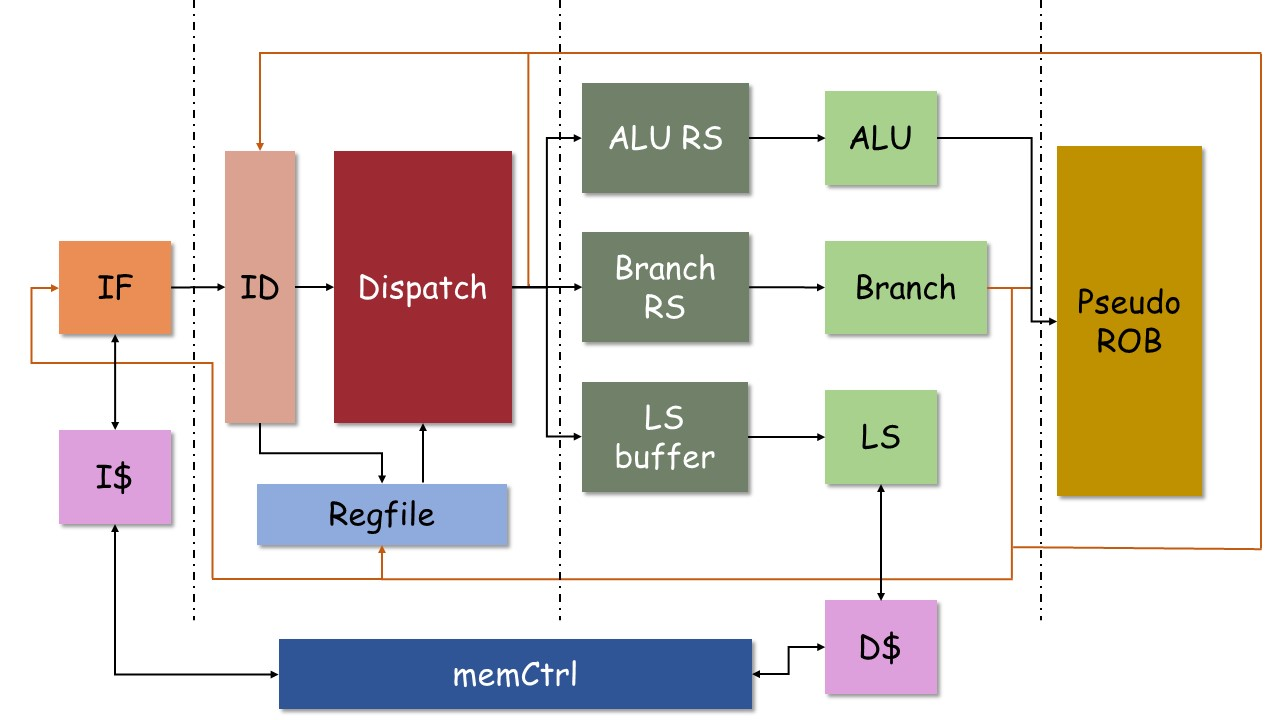
\includegraphics[width=120mm]{design.jpg}
 \end{figure}
\end{frame}

\begin{frame}[containsverbatim]{Branch Mask and Shadow Regfile}
    Consider the following code:
    \\[3mm]
\begin{lstlisting}[language=C,basicstyle=\footnotesize\consolas]
      lw  r10 0(r5)      #mask: 000
      bne r11 r12 jump;  #mask: 000, branch num:0
      add r10 r13 r14;   #mask: 001, so mask[0]=1
      ...
jump: add r11 r10 r12    #mask: 000
\end{lstlisting}

    The jump needs to know it should receive from the "lw r10 0(r5)" instead of "addi r10 r13 r14"
    \\[3mm]
    Just like a stack: \\
    ---------------------------------------------------------------------\\
    |data tag1 (branch free,lw) tag2 (branch num0,add r10)\\
    ---------------------------------------------------------------------\\
\end{frame}

\begin{frame}{Branch Mask}
    \begin{itemize}
        \item The reason why ALUrs and regfile so large is mainly logic for branch. 
    \end{itemize}
    \begin{figure}
    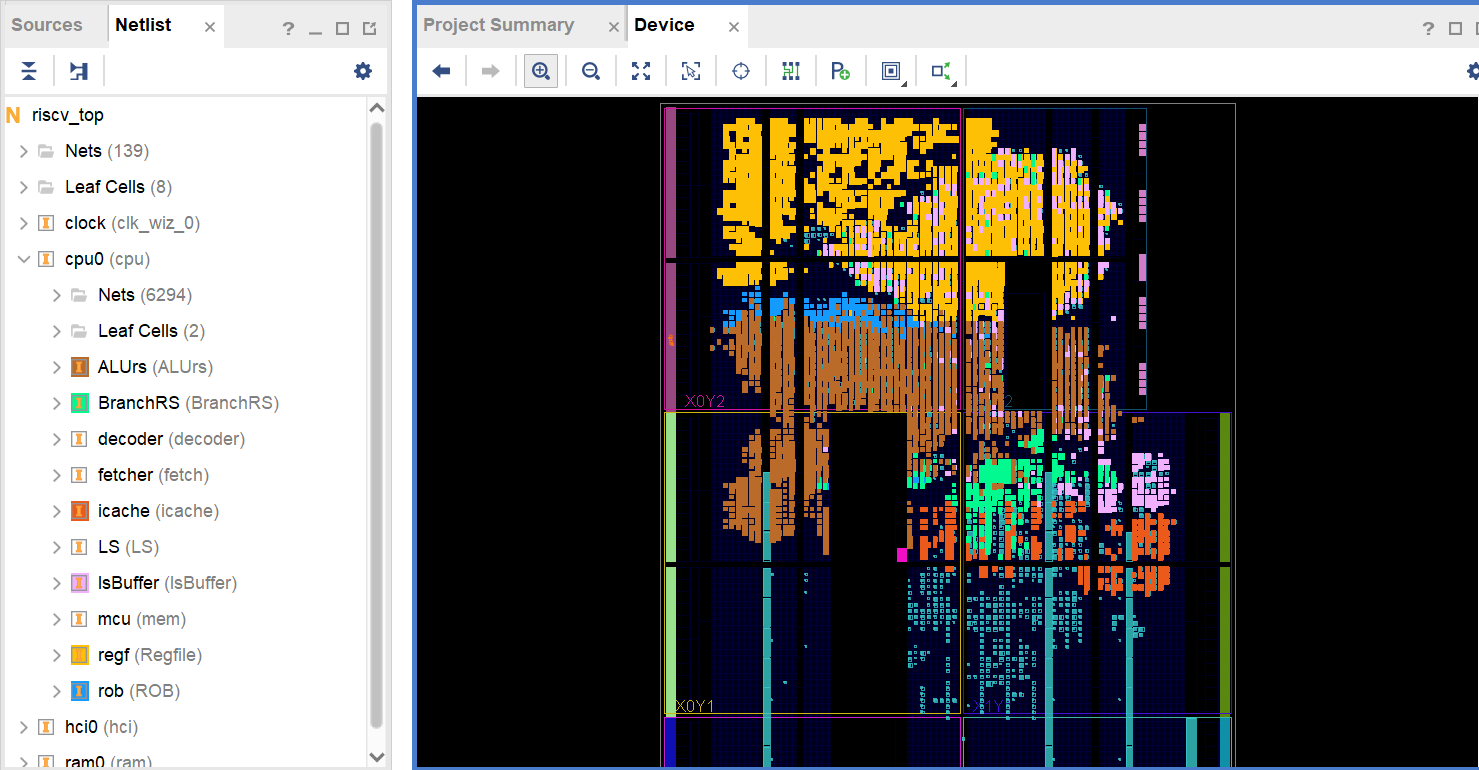
\includegraphics[width=110mm]{figure.png}
    \end{figure}
\end{frame}

\section{Pitfall}
\begin{frame}{Sometimes bigger and dumber is better?}
    Pitfall, according to CAAQA ed.6, chapter three. 
    \begin{itemize}
        \item Simply adding ROB line or RS has no improvement; 
        \item It costs a lot to enlarge the shadow page but is obviously useless. 
        \\[3mm]
        However, 
        \\[3mm]
        \item Enlarging the Cache seems useless, due to the limited testbench. 
        (admitting that meeting the testbench is the most important for a design)
        
        Itanium 2(well, it is also a failure) and i7 vs. Pentium 4. 
        \item Small cache may lead to worse performance(even write back)
        
        Load and replace, then done. So wait for a load more. 
    \end{itemize}
\end{frame}

\begin{frame}{And sometimes smarter is better than bigger and dumber?}
    Pitfall, according to CAAQA ed.6, chapter three. Really? 
\begin{itemize}
    \item The story of write-back dCache. 
    
    However: 

    \item The result of branch masks; 
    \item The result of special judge when entering RS and ROB. $\star\star\star$
            
    posedge 1: ID; \\
    posedge 2: in RS, then ready; (can let it work here)\\
    posedge 3: notice ready so do it;
\end{itemize}
    CAAQA mentions to consider the situation. 
\end{frame}

\section{Story}
\begin{frame}{My path}
    \begin{itemize}
        \item Learn and design;(6th Sep - 1st assignment)
        \item One without ROB first; 
        (after python interpreter - 23rd Nov, debug till 5th Dec)
        \item Add ROB, branch policy is stall; (23rd Nov - 9th Dec)
        \item Add branch mask, then make ROB a pseudo one to simplify. 
        Shadow regfile also;(till 15th Dec) 
        \item Add Dcache and Gshare. (1st Jan - 2nd Jan)
    \end{itemize}
\end{frame}

\begin{frame}[containsverbatim]{More stories}
    \begin{itemize}
        \item Shadow register again: No shadow data: $99\%\rightarrow50\%$ LUT; \\
        remark: considering the most complex logic, instead of the largest reg. (FF is no more than 20\%)
        \item Misprediction judgement; (more LUT but not very, 1ns less delay)
        \item Not assign a=b, simply use b; (not elegant, but 0.7ns less delay)
        \item Only control Enable signal strictly and others loosely. 
    \end{itemize}
\begin{lstlisting}[language=Verilog,
    keywordstyle=\color{blue!70}, 
    commentstyle=\color{red!50!green!50!blue!50}, 
    basicstyle=\footnotesize\consolas] 
    finalAddr = (op1 < op2) ? jumpAddr : nxtAddr;
    assign mispredict = (finalAddr == jumpAddr) ^ predict;
    //v.s.
    begin
        finalAddr = (op1 < op2) ? jumpAddr : nxtAddr;
        mispredict = (op1 < op2) ^ predict;
    end
\end{lstlisting}
\end{frame}

\section{Remark}
\begin{frame}{How to judge a design?}
    \begin{itemize}
        \item testbench? 2.2-2.25s for pi under 80MHz, delay is positive. 
        
        -actually not enough this time(still wrong once after passing);
        \item CPI? 
        
        -bad design can have good CPI but low frequency;

        \item Max Frequency and CPI? 
        
        -based on the tech of chip creation. 

        -1950s and early 1960s did not need Tomasulo. 
    \end{itemize}
    So what is this project for? A 1960 CPU or a 2020 CPU? Is Tomasulo a 2020 CPU? Remind Pentium 4. 
\end{frame}

\section{end}
\begin{frame}
\Huge{\centerline{Thanks}}
\end{frame}

\end{document}

